\subsection{引理 1 的证明}

设 \(\mathrm{E}_{s,s'}^*\) 是平面 \(\mathrm{E}_{s,s'} = \mathbf{Re}_s\oplus \mathbf{Re}_{s'}\) （第 2 号）的对偶。单射 \(\mathrm{E}_{s,s'}\to \mathrm{E}\) 的转置是一个满射

\[
p: \mathrm{E} ^ {*} \to \mathrm{E} _ {s, s ^ {\prime}} ^ {*}
\]

它与群 \(W_{s,s'}\) 的作用交换。显然，\(A_{s}\) 、\(A_{s'}\) 与 \(A_{s} \cap A_{s'}\) 是 \(E_{s,s'}^{*}\) 中相应子集（视为 Coxeter 群 \(W_{s,s'}\) 的逆步表示的空间）在 p 下的原像。此外，由于 \(W_{s,s'}\) 中元素的长度关于 \(\{s,s'\}\) 与关于 S 相同（第 IV 章，§1，第 8 号），我们最终可化归到 \(S = \{s,s'\}\) 的情形；若 \(m = m(s,s')\) ，则群 W 是 2m 阶的二面体群。

我们现在区分两种情形：

\begin{enumerate}
\def\labelenumi{\alph{enumi})}
\tightlist
\item
  \(m = +\infty\) .
\end{enumerate}

设 \((\varepsilon, \varepsilon')\) 是 \((e_s, e_{s'})\) 的对偶基。则

\[
s. \varepsilon = - \varepsilon + 2 \varepsilon^ {\prime}, s ^ {\prime}. \varepsilon = \varepsilon ,
\]

\[
s. \varepsilon^ {\prime} = \varepsilon^ {\prime}, s ^ {\prime}. \varepsilon^ {\prime} = 2 \varepsilon - \varepsilon^ {\prime}.
\]

设 D 是 \(E^{*}\) 中包含 \(\varepsilon\) 与 \(\varepsilon'\) 的仿射直线；上面的公式表明 D 在 s 与 \(s'\) 下稳定，且 s（分别为 \(s'\) ）在 D 上的限制是关于点 \(\varepsilon'\) （分别为 \(\varepsilon\) ）的反射。设

\[
\theta : \mathbf {R} \to \mathrm{D}
\]

是仿射双射 \(t \mapsto \theta(t) = t\varepsilon + (1 - t)\varepsilon'\) 。设 \(I_n\) 为 \(\theta\) 作用于开区间 \(]n, n + 1[\) 所得的像，并设 \(C_n\) 为诸 \(\lambda I_n\) （\(\lambda > 0\) ）的并。则 \(C_0 = C\) ；此外，把 §2 第 4 号的注应用于仿射空间 D，诸 \(I_n\) 被 W 简单传递地置换；从而诸 \(C_n\) 亦然。若 \(v \in W\) ，则 \(v(C)\) 等于某个 \(C_n\) ，从而含于 \(A_s\) （当 \(n \geqslant 0\) 时）或 \(s(A_s)\) （当 \(n < 0\) 时）。在第二种情形，\(I_0\) 与 \(I_n\) 位于点 \(\varepsilon'\) 的两侧；从而 \(l(sv) = l(v) - 1\) （出处同前）。

\begin{enumerate}
\def\labelenumi{\alph{enumi})}
\setcounter{enumi}{1}
\tightlist
\item
  m 是有限的。
\end{enumerate}

于是型 \(B_{M}\) 非退化（第 2 号），从而我们可以把 \(E^{*}\) 与 E 等同起来。我们已经看到，可以给 E 定向，使得半直线 \(R_{+}e_{s}\) 与 \(R_{+}e_{s'}\) 之间的角等于 \(\pi - \frac{\pi}{m}\) 。设 D（分别为 \(D'\) ）是由 \(R_{+}e_{s}\) （分别为 \(R_{+}e_{s'}\) ）经 \(\pi/2\) （分别为 \(-\pi/2\) ）的旋转得到的半直线，参见~图 2。室 C 是由 \(x \in E\) （其与 \(e_{s}\) 及 \(e_{s'}\) 的标量积 \textgreater0 ）所成的集合；这是以 \(D'\) 为始边、以 D 为终边的开角扇区。由 §2 第 5 号的注，W 的每个元素 v 把 C 变成一个与 C 位于 D 同侧的角扇区（即含于 \(A_{s}\) ）或位于 D 异侧的角扇区（即含于 \(s(A_{s})\) ），并且在后一情形

\[
l (s v) = l (v) - 1,
\]

这就完成了引理的证明。

\pandocbounded{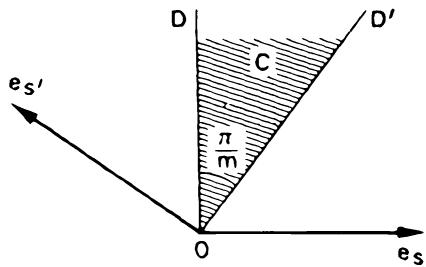
\includegraphics[keepaspectratio]{images/part001_dfbe6528.jpg}}\\
图 2

